	\paragraph{QuizziPedia::Front-End::Directives::EmptySpaceAnswerDirective}
		
		\label{QuizziPedia::Front-End::Directives::EmptySpaceAnswerDirective}
		
		\begin{figure}[ht]
			\centering
			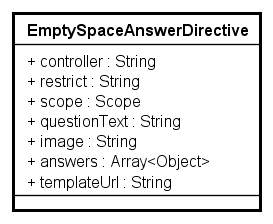
\includegraphics[scale=0.80,keepaspectratio]{UML/Classi/Front-End/QuizziPedia_Front-end_Templates_EmptySpaceAnswerTemplate.png}
			\caption{QuizziPedia::Front-End::Directives::EmptyChoiceAnswerDirective}
		\end{figure} \FloatBarrier
		
		\begin{itemize}
			\item \textbf{Descrizione}: rappresenta il componente grafico che permette all'utente di visualizzare l'esercizio a riempimento di spazi vuoti. Viene visualizzato dinamicamente all'interno delle views \texttt{TrainingView} e \texttt{FillingQuestionnaireView} mediante il controller \texttt{QuestionsController};
			\item \textbf{Utilizzo}: viene utilizzato per consentire all'utente la compilazione dell'esercizio a riempimento di spazi vuoti;
			\item \textbf{Relazioni con altre classi}: 
			\begin{itemize}
				\item \textit{IN} \texttt{QuestionsModelView}: classe di tipo modelview la cui istanziazione è contenuta all'interno della variabile di ambiente \$scope di \textit{Angular.js\ped{G}}. All'interno di essa sono presenti le variabili e i metodi necessari per il \textit{Two-Way Data-Binding\ped{G}} tra le directive che compongono dinamicamente la vista della domanda e il controller \texttt{QuestionsController};
				\item \textit{OUT} \texttt{TrainingView}: view principale della modalità allenamento. Conterrà i vari templates di ogni domanda dell'allenamento;
				\item \textit{OUT} \texttt{FillingQuestionnaireView}: view principale per la compilazione del questionario; conterrà i vari templates di ogni domanda appartenente al questionario;   
				\item \textit{IN} \texttt{LangModel}: rappresenta il modello delle informazioni per la giusta traduzione dell'applicazione.
			\end{itemize}
			\item \textbf{Attributi}: 
			\begin{itemize}
				\item \texttt{+ questionText: String} \\ Identifica il testo della domanda;
				\item \texttt{+ image: String} \\ Identifica l'url di una possibile immagine nella domanda;
				\item \texttt{+ answers: Array[Object]} \\ Array che contiene coppie di valori. Queste coppie sono formate da:
				\begin{itemize}
					\item \texttt{+ type: String} \\ Indica la tipologia della risposta;
					\item \texttt{+ text: String} \\ Contiene il testo dell'affermazione;
					\item \texttt{+ url: String} \\ Rappresenta l'immagine della risposta;
					\item \texttt{+ attributesForEmptySpaces: Mixed} \\ Contiene i seguenti attributi:
					\begin{enumerate}
						\item \texttt{+ wordNumber: Number} \\ Rappresenta la posizione dello spazio vuoto in cui deve andare inserita la parola.
					\end{enumerate}
				\end{itemize}
				\item \texttt{+ controller: String} \\ Stringa contenente il nome del controller della direttiva;
				\item \texttt{+ restrict: String} \\ Stringa che permette di definire le modalità di inserimento della direttiva all'interno della pagina;
				\item \texttt{+ scope: Scope} \\Oggetto \texttt{\$scope} interno della direttiva, contiene le funzionalità per gestire i dati presenti all'interno;
				\item \texttt{+ templateUrl: String}: stringa contenente il percorso del file \textit{HTML\ped{G}} che contiene la direttive.
			\end{itemize}
		\end{itemize}